
\documentclass{ieeeaccess}

\usepackage{cite}
\usepackage{amsmath,amssymb,amsfonts}
\usepackage{graphicx}
\usepackage{textcomp}
\usepackage{xcolor}
\usepackage{booktabs}
\usepackage{multirow}
\usepackage{url}
\usepackage{hyperref}

\newcommand{\orcidlink}[1]{\href{https://orcid.org/#1}{\raisebox{-0.25ex}{
\includegraphics[height=1.7ex]{figures/orcid.pdf}}}}
\usepackage{etoolbox}
\NewSpotColorSpace{PANTONE}
\AddSpotColor{PANTONE} {PANTONE3015C} {PANTONE\SpotSpace 3015\SpotSpace C} {1 0.3 0 0.2}
\SetPageColorSpace{PANTONE}
\usepackage{bm}
\makeatletter
\AtBeginDocument{\DeclareMathVersion{bold}
\SetSymbolFont{operators}{bold}{T1}{times}{b}{n}
\SetSymbolFont{NewLetters}{bold}{T1}{times}{b}{it}
\SetMathAlphabet{\mathrm}{bold}{T1}{times}{b}{n}
\SetMathAlphabet{\mathit}{bold}{T1}{times}{b}{it}
\SetMathAlphabet{\mathbf}{bold}{T1}{times}{b}{n}
\SetMathAlphabet{\mathtt}{bold}{OT1}{pcr}{b}{n}
\SetSymbolFont{symbols}{bold}{OMS}{cmsy}{b}{n}
\renewcommand\boldmath{\@nomath\boldmath\mathversion{bold}}}
\makeatother

\def\BibTeX{{\rm B\kern-.05em{\sc i\kern-.025em b}\kern-.08em
    T\kern-.1667em\lower.7ex\hbox{E}\kern-.125emX}}

\history{Date of publication xxxx 00, 0000, date of current version xxxx 00, 0000.}
\doi{10.1109/ACCESS.2024.0429000}
\headname{Research Article}

\begin{document}

\title{From Hand-Drawn Schematics to SPICE Netlists: A Deterministic Pipeline with Endpoint-Graph Wire Joining and a Human-Verified Connectivity Benchmark}

% ORCID: add each author's ORCID before submission, e.g.
%   \uppercase{Bosco Chanam}\authorrefmark{1}~\orcidlink{0000-0000-0000-0000}
\author{\uppercase{Bosco Chanam}\authorrefmark{1}~\orcidlink{0009-0009-2527-0967},
\uppercase{Chris Dcosta}\authorrefmark{1}~\orcidlink{0009-0007-7295-0573},
\uppercase{Pranavesh Kumar Talupuri}\authorrefmark{2}~\orcidlink{0009-0005-8974-2012},
\uppercase{Shwetambari Chiwhane}\authorrefmark{1}~\orcidlink{0000-0002-3534-9654},
\uppercase{Ashay Kumar Singh}\authorrefmark{1}~\orcidlink{0009-0004-9105-7383},
and \uppercase{Arghadeep Das}\authorrefmark{1}~\orcidlink{0009-0000-9207-7694}}
\address[1]{Symbiosis Institute of Technology, Pune 412115, India (e-mail: boscochanam@gmail.com; chrisdcosta777@gmail.com; shwetambari.chiwhane@sitpune.edu.in; ashay.sit@gmail.com; arghadeep.das.work@gmail.com)}
\address[2]{Department of Computer Science, University of Southern California, Los Angeles, CA 90089 USA (e-mail: talupuri@usc.edu)}
\tfootnote{This work received no external funding.}

\markboth
{Chanam \headeretal: From Hand-Drawn Schematics to SPICE Netlists}
{Chanam \headeretal: From Hand-Drawn Schematics to SPICE Netlists}

\corresp{Corresponding author: Bosco Chanam (e-mail: boscochanam@gmail.com).}

\begin{abstract}
Digitizing a hand-drawn circuit schematic into a SPICE-format netlist is hard mainly because connectivity recovery breaks down under noisy wire detections. We present a deterministic pipeline that turns a scanned schematic into a structural SPICE-format netlist: component detection, an occlusion-first wire extractor, and a graph-based join that resolves electrical connectivity. Component values are not read from the image; they come from the user or a downstream value-reader. The core contribution is the join itself: an endpoint-graph model over wire endpoints and component pins with five edge types, paired with degree-budget completion that recovers dropped connections through min-cost $b$-matching while bounding over-merge with per-pin budgets and self-loop guards. We also introduce a synthetic perturbation protocol and, to our knowledge, the first human-verified net-level connectivity benchmark for hand-drawn circuits, covering 31 images from CGHD-1152. The occlusion-first extractor reaches wire-detection F1~=~0.976 on 134 scanned images. On the 31-image human-verified benchmark, the best join reaches connectivity micro-F1~=~0.890, ahead of the prior completion default (0.83), a legacy radius union-find join (0.67), a connected-component net-tracing baseline (0.62), and a Hough-plus-proximity line tracer (0.81), all evaluated on identical detected wires. Running the same join on perfect wire labels does not raise micro-F1, which means connectivity, not wire detection, is the bottleneck. A first-party comparison shows a strong vision-language model reaching 0.923 on the same images: statistically indistinguishable from our join, but far more expensive and without structural guarantees. That result argues for explicit geometric connectivity recovery in a deployable digitizer.
\end{abstract}

\begin{keywords}
circuit digitization, connectivity benchmark, graph-based connectivity, hand-drawn circuits, image-to-netlist, netlist extraction, schematic recognition, SPICE, wire extraction, wire joining
\end{keywords}

\titlepgskip=-21pt

\maketitle

\begin{figure*}[t]
\centering
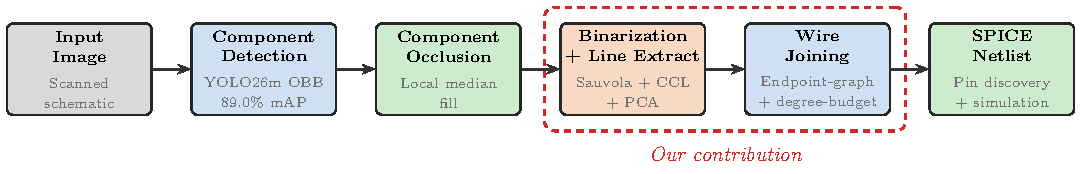
\includegraphics[width=\textwidth]{figures/pipeline_overview.pdf}
\caption{End-to-end pipeline for digitizing a scanned circuit diagram. Our contributions span the wire extraction and joining stages; the join (dashed red) decides which extracted wire segments connect to which component pins, and it is the dominant failure mode in end-to-end digitization.}
\label{fig:pipeline}
\end{figure*}

\begin{figure*}[t]
\centering
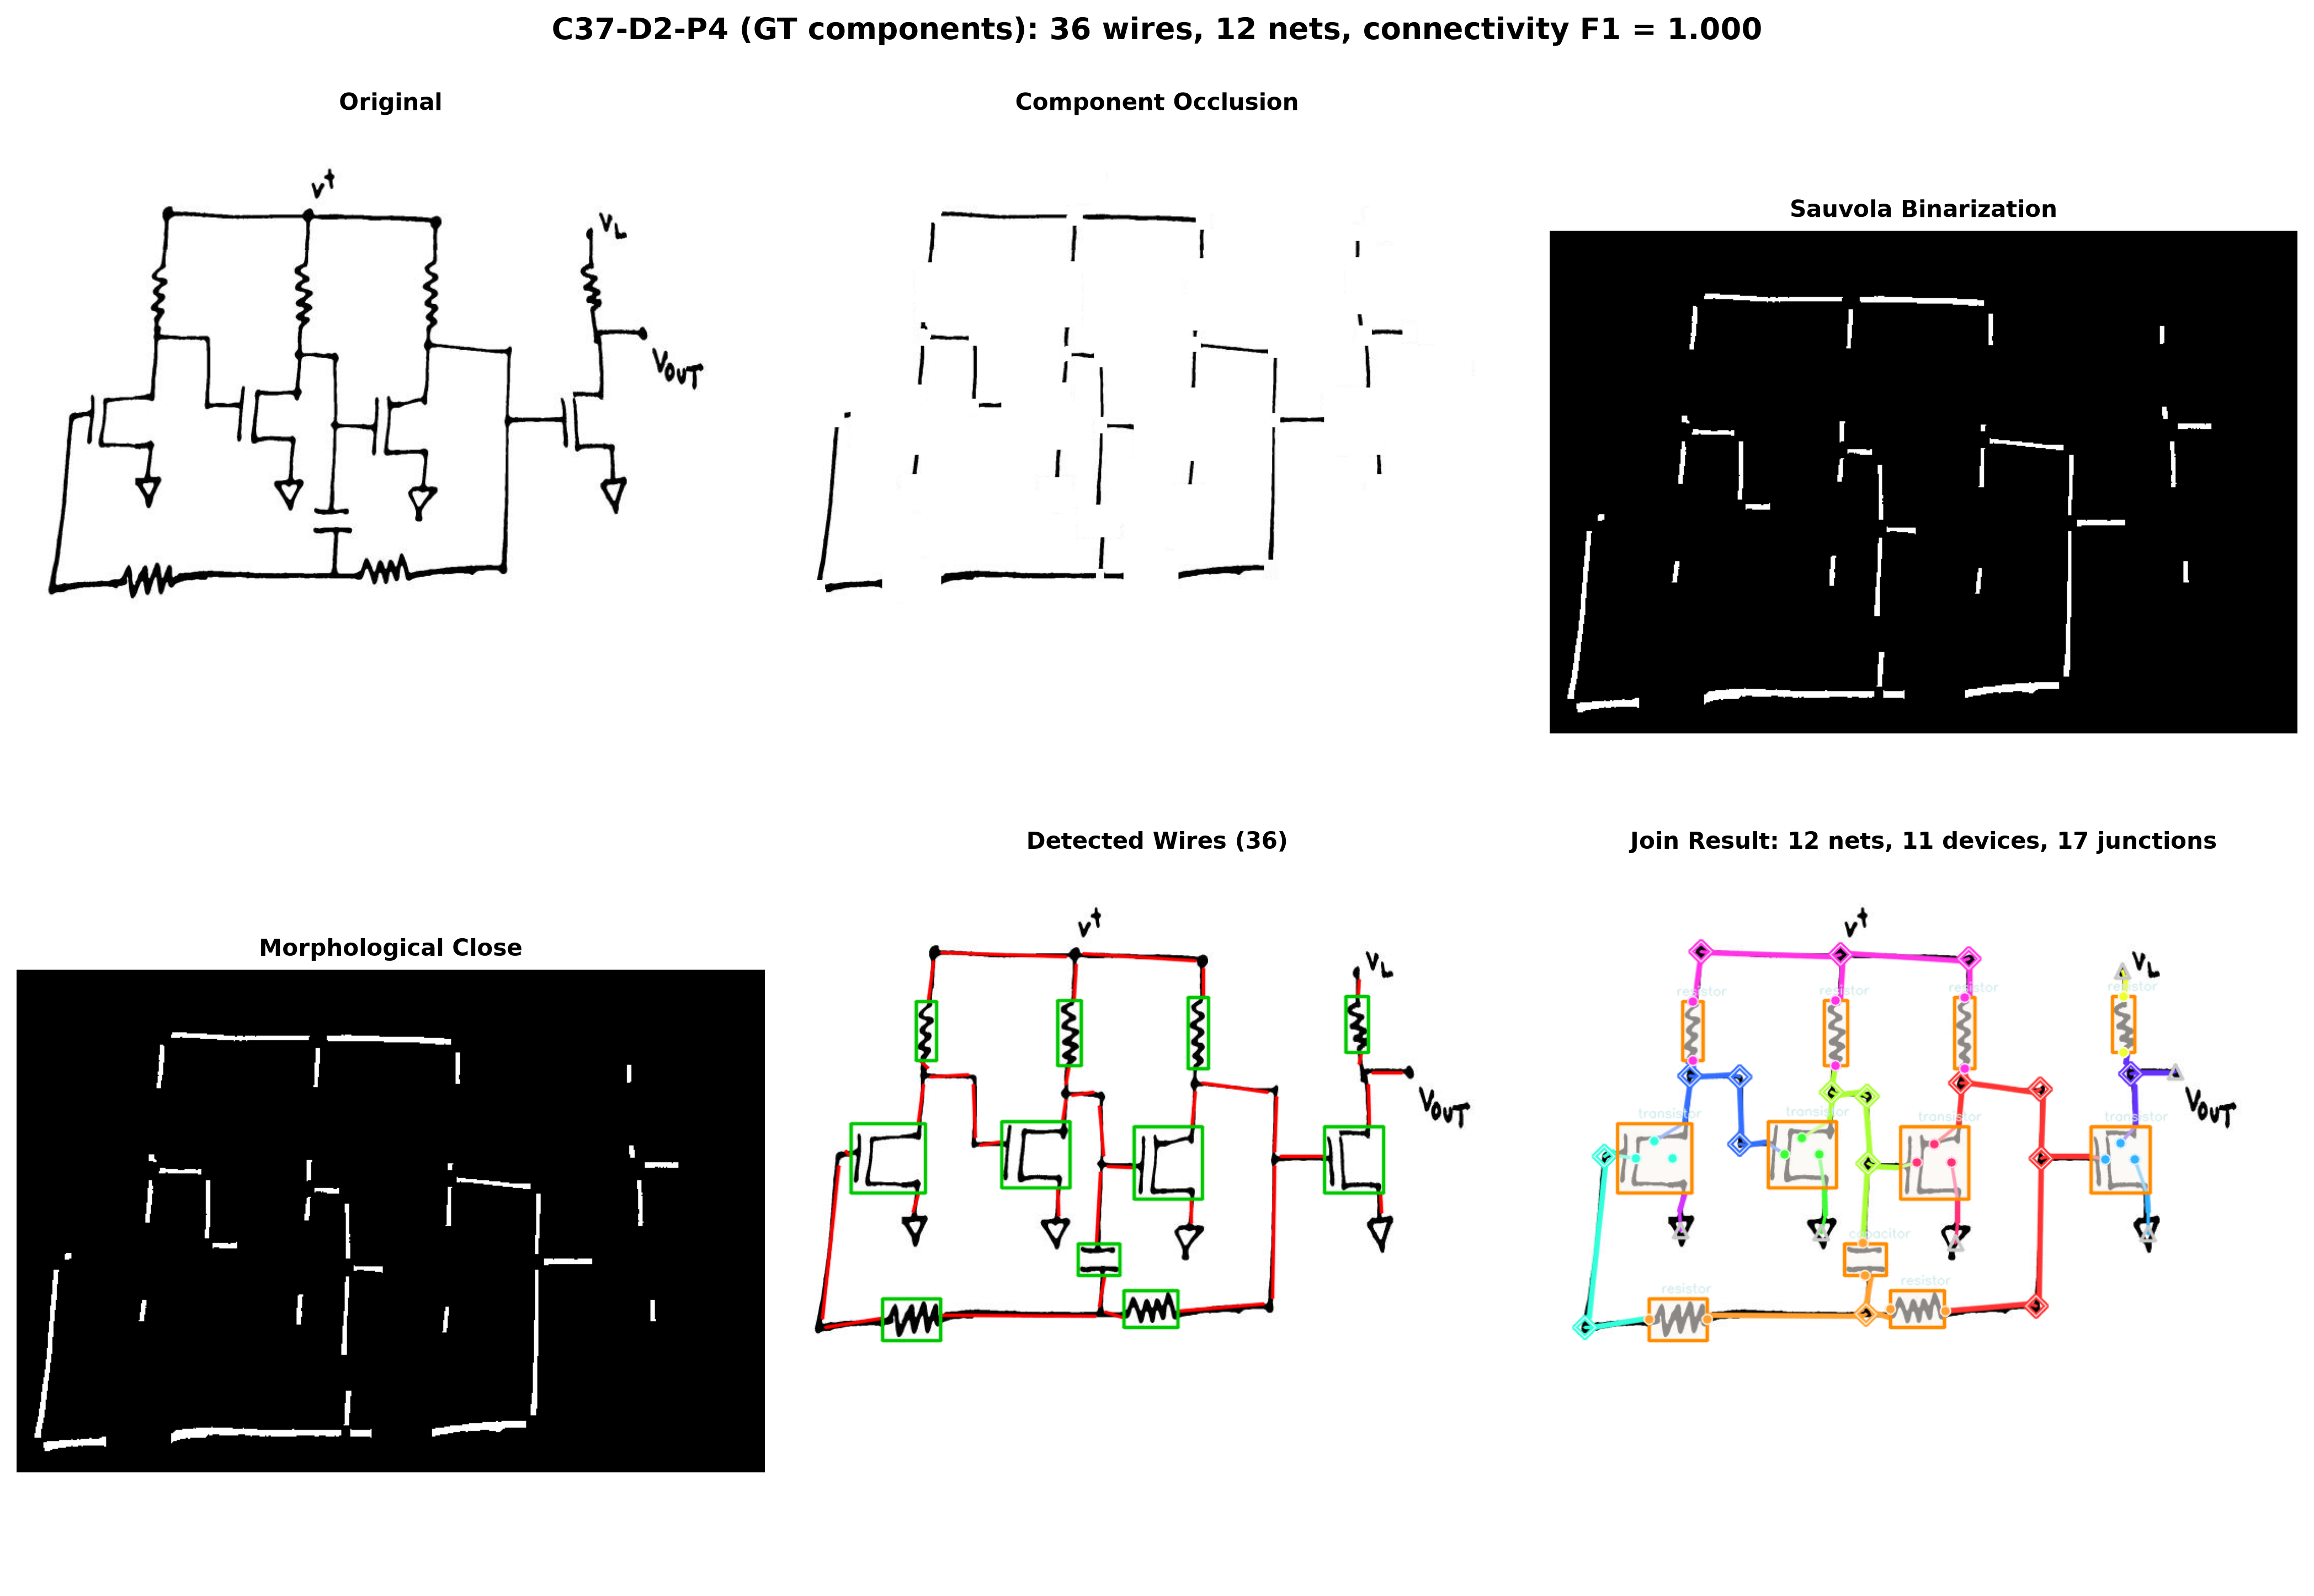
\includegraphics[width=0.48\textwidth]{figures/pipeline_examples/C37-D2-P4-jpg.png}
\hfill
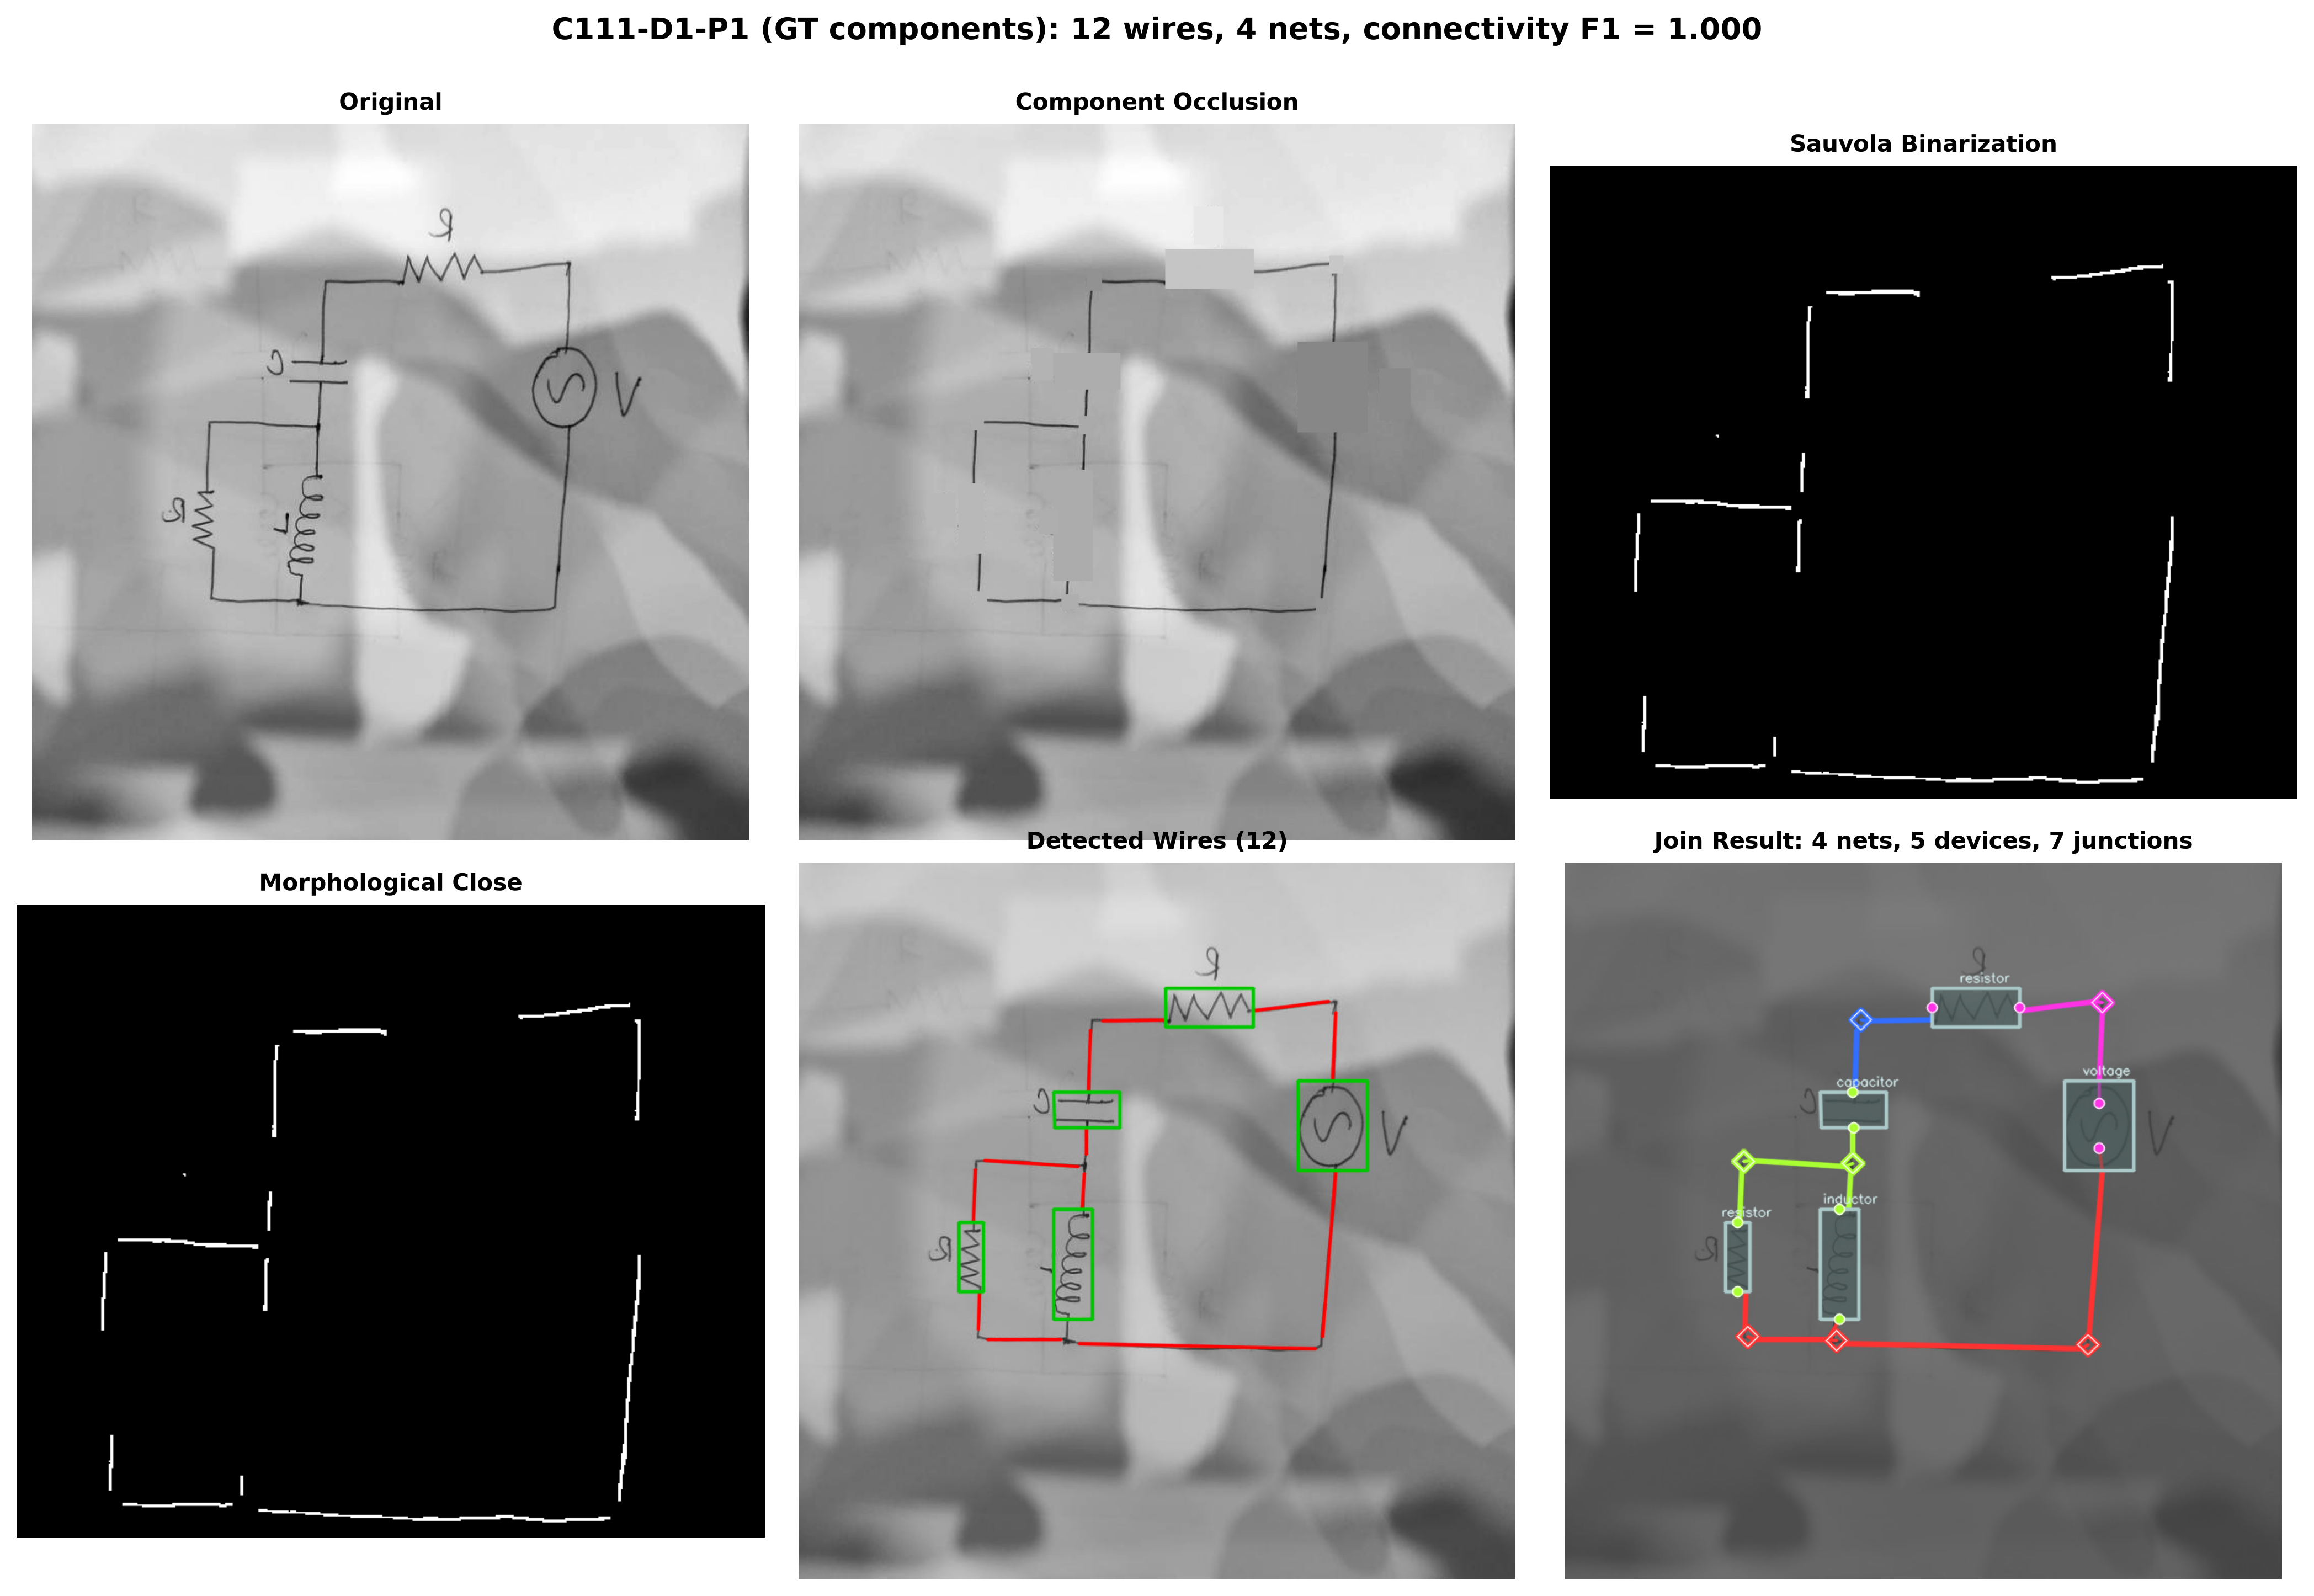
\includegraphics[width=0.48\textwidth]{figures/pipeline_examples/C111-D1-P1-jpg.png}
\caption{Pipeline stages on two real hand-drawn circuit images, joined with our scale-relative completion join (connectivity F1~=~1.000 on both). Left: a four-transistor analog cell (35 wires, 7 nets). Right: an RLC loop photographed on a textured surface (11 wires, 4 nets). Each panel shows, in order, the original scan, component occlusion, Sauvola binarization, morphological close, detected wires (red overlay), and the join result. In the join result every recovered net is a distinct colour drawn along its conductors; component bounding boxes are the ground-truth labels (used throughout the net-level evaluation to isolate the join), filled dots are device pins, diamonds mark junctions, and triangles mark terminals and ground.}
\label{fig:pipeline_examples}
\end{figure*}

\section{Introduction}

An analog schematic packs component types, values, and topology into a drawing meant for a human reader. Converting a scanned schematic into a machine-readable SPICE (Simulation Program with Integrated Circuit Emphasis) netlist opens the door to automated simulation, design verification, and circuit analysis at scale. Component recognition has become reliable as object detection has improved, but the \emph{joining} problem, working out which wire segments connect to which component pins and to each other, is still the main failure mode in end-to-end digitization.

Three things make this hard. Wire endpoints pulled from a binarized image are noisy by nature: the same circuit, drawn by different people, produces endpoint positions that vary by 10--80 pixels. Component bounding boxes overlap wire endpoints, so it is often unclear whether an endpoint touches a pin or is just passing nearby. And T-junctions, collinear fragments, and crossing wires create connectivity patterns that a simple radius-based rule cannot resolve without merging things that should stay separate.

One obvious alternative is to hand the schematic to a large vision-language model (VLM) and let it emit a netlist directly. We test this in Section~\ref{sec:vlm_results}: a strong VLM reaches connectivity accuracy statistically indistinguishable from our geometric pipeline, but at orders-of-magnitude higher cost, and it returns free-form text rather than a structured netlist, gives no structural guarantee against electrically invalid output (a shorted two-terminal part, say), and drops connections on the most complex circuits. That combination is the case for an explicit, inspectable geometric pipeline: one whose output is a netlist by construction, matches the VLM's accuracy, and stays deterministic and structurally valid.

Our pipeline addresses all three problems with three new pieces: (1)~an \emph{occlusion-first wire extractor} that masks detected components before binarization and estimates per-segment endpoints, giving a line-segment-with-endpoints representation, rather than tracing nets directly into connected components as prior systems do, which is what makes graph-based joining possible in the first place; (2)~an \emph{endpoint-graph join} that builds a graph over both wire endpoints and component pins with five edge types, each capturing a distinct connectivity pattern; and (3)~a \emph{degree-budget completion} algorithm that finds and reconnects dropped connections through constrained optimization. We evaluate the pipeline on the CGHD-1152 dataset~\cite{bayer2021cghd}, using a synthetic error-injection framework for systematic robustness analysis and a human-verified net-level benchmark for real-image validation.

\section{Related Work}

Schematic-to-netlist conversion has moved quickly. Kelly and Cole~\cite{kelly2024digitizing} built a pattern-recognition workflow for digitizing circuit schematics that combines optical character recognition (OCR) for component values with network-graph construction, reporting an 86.4\% success rate. SINA~\cite{sina2026} is the closest contemporary system: it pairs a YOLOv11 detector with connected-component labeling (CCL) and OCR, calls a vision-language model (VLM) only for reference-designator assignment, and reports 96.47\% netlist-generation accuracy, a 2.72$\times$ improvement over the prior state of the art. SINA keeps the VLM out of connectivity and derives nets from CCL proximity instead, a design choice we also make (Section~\ref{sec:vlm_connectivity}). Masala-CHAI~\cite{masalachai2024} (Auto-SPICE) uses large language models to produce SPICE netlists from analog schematics at scale. The concurrent work of Peker et al.~\cite{peker2026} (IEEE Access, 2026) is the closest match to our setting: a fully automated image-to-SPICE pipeline for printed and hand-drawn transistor-level circuits that pairs YOLOv8/11 detection with a \emph{contour-based} node-detection module (components are erased and nets are read off the contours of the residual wire pixels), and, like us, validates netlists by automated LTspice simulation against a reference. On their in-house seven-topology MOSFET dataset they report 93.33\% (printed) and 85.33\% (hand-drawn) whole-netlist success. Their node detector is one instance of the connected-component/contour recipe we test as a baseline (Section~\ref{sec:real_eval}); their dataset (transistor-level analog, authored in-house) and metric (LTspice node-voltage pass/fail) differ enough from ours (discrete components on CGHD-1152, component-pair F1) that the headline numbers do not compare directly, but the pairing does show that contour/CCL node detection is still the dominant approach, and our endpoint-graph join clearly beats it on a controlled, identical-input benchmark. Instance-segmentation methods take a different route, extracting circuit graphs straight from pixels: Bayer et al.~\cite{instanceseg2023} segment components and wires for graph extraction over the CGHD lineage. For hand-drawn input specifically, object-detection pipelines~\cite{handdrawn2021} and the recent JUHCCR-v1 database~\cite{juhccr2025} target component recognition on freehand sketches. Most of this work builds on general-purpose object detectors such as the YOLO family~\cite{redmon2016yolo,jocher2023yolo} and OCR engines such as Tesseract~\cite{smith2007tesseract}, aiming ultimately at simulator-ready output in formats such as SPICE~\cite{nagel1973spice}. Taken together, these results treat detection and recognition as largely solved problems; the open problem is reconstructing electrical connectivity, which is what we address here.

None of this works without annotated data. The CGHD hand-drawing dataset~\cite{bayer2021cghd} supplies component- and wire-level annotations for handwritten schematics. In the analog/mixed-signal (AMS) space, AMSnet~2.0~\cite{amsnet2025} offers a large database built with AI-assisted segmentation for net detection, and AMSBench~\cite{amsbench2025} benchmarks multimodal LLM capability across AMS circuit tasks. Outside circuits, DiagramNet~\cite{diagramnet2026} contributes an end-to-end framework and dataset for non-standard system-level diagrams, with an explicit connection-recognition task scored by F1. These benchmarks show where current systems already work (component recognition) and where they do not (connectivity); we add to that picture with a synthetic robustness protocol that isolates the join step under controlled detector noise.

\label{sec:vlm_connectivity}
General-purpose VLMs and LLMs have found broad use in electronic design~\cite{llm4eda2024} and, more specifically, in circuit understanding. Kulkarni et al.~\cite{kulkarni2025enhancing} proposed Near Sight Correction using VLMs, reporting 87.4\% accuracy on circuit visual question answering (VQA) and 0.87 F1 on connection-matrix prediction. But several independent benchmarks agree that general VLMs are much better at component recognition than at connectivity. On the DiagramNet connection task~\cite{diagramnet2026}, leading general models score very low F1 (GPT-5 at 0.029, Claude-Sonnet-4 at 0.265, and Gemini-2.5-Pro at 0.008), while a task-tuned 3B model reaches 0.735. AMSBench~\cite{amsbench2025} finds a similar gap for MLLMs on AMS connectivity. This supports a design choice we share with SINA~\cite{sina2026}: keep wire-to-component connectivity out of the VLM and solve it with an explicit geometric model instead. We make that separation concrete and quantify it with our own Claude-VLM connectivity experiment.

Classical wire extraction leans on edge detection, morphological operations, and the Hough transform~\cite{duda1972hough}, usually after adaptive binarization such as Sauvola thresholding~\cite{sauvola2000} and connected-component labeling~\cite{he2017ccl}. Most existing pipelines join wires by radius-based proximity: each wire endpoint grabs every component pin within a fixed threshold (typically 30px), and the result is stitched together with transitive union-find~\cite{tarjan1975union}. When several components fall inside that threshold, the radius rule over-merges and shorts two-terminal parts (R, C, L, D) onto a shared net. SINA~\cite{sina2026} derives nets from CCL proximity, which carries the same vulnerability under detector noise. We instead treat joining as a typed endpoint graph that folds in component geometry and directional preference, and clean up what is left with degree-budget completion: a bounded $b$-matching formulation~\cite{kuhn1955,schrijver2003combinatorial} that caps per-pin degree and so limits over-merge when endpoints are dropped or displaced. This is a different animal from graph neural networks for netlist reverse engineering~\cite{alrahis2021gnn}, which learn representations over gate-level graphs that have already been extracted; our graph is purely geometric, with edges that encode spatial relationships between wire endpoints and component pins. A newer, complementary direction swaps rule-based connectivity for a learned model: Netlistify~\cite{netlistify2025} predicts terminal connectivity with a Transformer and reports a 12.4\% F1 gain over AMSnet on printed AMS schematics. Models like this are capable but need task-specific connectivity training data, and, trained on printed schematics, they do not transfer to hand-drawn images without retraining; our geometric model needs no connectivity training at all, which is the point of building it this way. Open hand-drawn efforts such as CircuitNet~\cite{circuitnet} take a similar traditional-image-processing route, pairing a classifier with a heuristic netlist generator.

\section{Method}

\subsection{Pipeline Overview}

Figure~\ref{fig:pipeline} lays out the six stages: (1)~component detection with an oriented bounding box (OBB) YOLO model; (2)~component occlusion, filling detected regions with local median color; (3)~Sauvola adaptive binarization; (4)~connected-component labeling with morphological post-processing; (5)~wire endpoint extraction via principal component analysis (PCA) on endpoint regions; and (6)~wire joining with the endpoint-graph model and degree-budget completion. The output is a netlist that maps component pins to electrical nodes, ready for SPICE netlist generation. Figure~\ref{fig:pipeline_examples} walks two representative circuits through each stage.

\subsection{Endpoint-Graph Join Model}

We are given a set of wire segments $\mathcal{W} = \{w_1, \ldots, w_m\}$ with endpoints $\text{ep}(w_i) = (a_i, b_i)$ and component pins $\mathcal{P} = \{p_1, \ldots, p_n\}$. From these we build an undirected graph $G = (V, E)$ with $V = \text{eps}(\mathcal{W}) \cup \mathcal{P}$.

\textbf{Edge type 1 (wire body):} For each wire $w_i$ we add edge $(a_i, b_i)$ with weight 0, so both endpoints of a wire always land in the same net.

\textbf{Edge type 2 (endpoint--endpoint):} For endpoint pairs $(e_i, e_j)$ with $\|e_i - e_j\| \leq \tau_{\text{join}}$, we add an edge with weight $\|e_i - e_j\|$, capturing wire fragments, corners, and junctions.

\textbf{Edge type 3 (endpoint--pin):} For each endpoint $e$ and pin $p$ with $\|e - p\| \leq \tau_{\text{pin}}$, we add an edge with weight $\|e - p\| \cdot (1 - \alpha \cdot \cos\theta)$, where $\theta$ is the angle between the wire direction and the endpoint-to-pin vector and $\alpha$ controls directional preference. This is the edge type that actually connects wires to components, and it does most of the work.

\textbf{Edge type 4 (endpoint--wire-body):} For each endpoint $e$ and wire segment $w_j = (c, d)$, if the point-to-segment distance $\text{dist}(e, w_j) \leq \tau_t$, we add an edge with weight $\text{dist}(e, w_j)$, capturing T-junctions where one wire terminates on another wire's body.

\textbf{Edge type 5 (pin--wire-body):} For each component pin $p$ and wire segment $w_j$, if the point-to-segment distance $\text{dist}(p, w_j) \leq \tau_t$ and the projection lands mid-span (not at $w_j$'s endpoints, which edge type 3 already handles), we add an edge with weight $\text{dist}(p, w_j)$. This binds a component that taps onto a passing rail along the wire's body rather than at its end, recovering connectivity that endpoint-only binding misses without the all-to-all over-merge that plain radius grabbing produces.

The tolerances $\tau_{\text{join}}$, $\tau_{\text{pin}}$, and $\tau_t$ are \emph{scale-relative}: $\tau = k \cdot s$, where $s$ is the characteristic scale (median component diagonal), so one parameter setting works across circuits of different sizes. Because $s$ is a single scalar per image, it does not model size variance within an image: a schematic that mixes a large IC with small discrete symbols shares one $\tau$ for both. In practice we also clamp the tolerances to a fixed pixel range (e.g.\ $\tau_{\text{pin}} \in [24, 60]\,$px and $\tau_t \in [8, 20]\,$px), which keeps the scale-relative rule from running away on circuits of extreme size.

\textbf{Component-first pin assignment:} For edge type 3 we assign pins in two steps. First, each endpoint is matched to its nearest component by bounding-box distance (zero if inside the bbox, with a generous radius of $\max(\tau_{\text{pin}}, 0.5 \cdot \text{diagonal})$). Second, within that component, we pick the pin by geometric position: for horizontal components ($w > h$), the left pin if endpoint $x <$ center $x$ and the right pin otherwise; for vertical components ($h > w$), the top pin if endpoint $y <$ center $y$ and the bottom pin otherwise. This handles the common case where an endpoint lands inside a component's bounding box but far from its actual pin. Figure~\ref{fig:endpoint_graph} contrasts the legacy radius join with our endpoint-graph model.

\begin{figure*}[t]
\centering
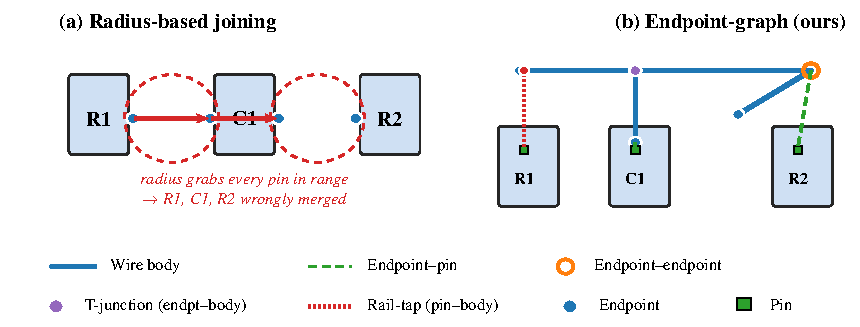
\includegraphics[width=\columnwidth]{figures/endpoint_graph.pdf}
\caption{Two joining approaches compared. (a)~Radius-based join (legacy): each wire endpoint grabs every pin within a fixed threshold, which causes over-merging. (b)~Our endpoint-graph model: typed edges (wire body, endpoint--pin) with directional preference resolve connectivity without over-merging.}
\label{fig:endpoint_graph}
\end{figure*}

Nets fall out as connected components of $G$, projected onto pins, giving a netlist that maps each pin to a net identifier.

\subsection{Degree-Budget Completion}

The endpoint-graph join can leave some component pins ``floating,'' touching only their own component's net with no wire reaching another component. That usually means the detector dropped a wire endpoint or placed it too far from the correct pin.

Degree-budget completion finds these floating pins and reconnects them through constrained optimization. A pin $p$ counts as floating if its net contains only pins from $p$'s own component, ignoring inert types such as gnd, vss, text, antenna, junction, and terminal. For each floating pin $p$ we generate candidate edges to every pin $q$ in other components within reach $r = \rho \cdot s$, where $\rho$ is the reach factor; the deployed scale-relative join uses $\rho = 4$, and Section~\ref{sec:real_eval} shows the F1 plateau is broad across $\rho \in [3,5]$. Candidate edge weight is Euclidean distance $\|p - q\|$. We then solve a min-cost $b$-matching problem, $\min \sum_{(p,q) \in E'} w(p,q) \cdot x_{pq}$ subject to $\sum_q x_{pq} \leq 1$ for each floating pin $p$, with the Hungarian algorithm~\cite{kuhn1955} (\texttt{scipy.optimize.linear\_sum\_assignment}). Each target pin offers up to three slots so a legitimate multi-terminal net is not starved, and a per-pin opt-out lets a pin with no good target stay unconnected rather than forcing a bad edge. Last, we reject any matched edge $(p, q)$ if $p$ and $q$ sit on the same component, or if the edge would merge two nets that already share a component, which structurally rules out short-circuiting a two-terminal part.

Completion edges are ``wireless'': they stand for inferred connections with no corresponding wire segment, much like a manual pin merge in a schematic editor. Figure~\ref{fig:completion} shows the completion step.

\begin{figure*}[t]
\centering
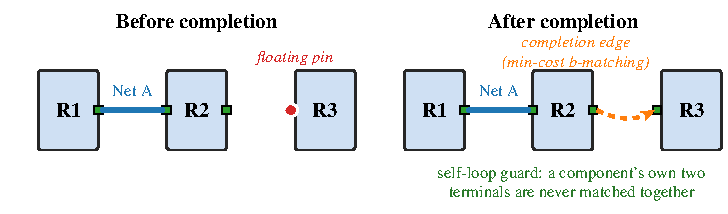
\includegraphics[width=\columnwidth]{figures/completion.pdf}
\caption{Degree-budget completion. Left: after base joining, some pins are ``floating,'' touching only their own component. Right: completion reconnects floating pins via min-cost $b$-matching (orange dashed); the self-loop guard prevents shorts within two-terminal components.}
\label{fig:completion}
\end{figure*}

\section{Results}

\subsection{Synthetic Evaluation Framework}

We hand-authored 15 synthetic circuits spanning 3--6 components and 2--6 nets: parallel resistors, series dividers, Wheatstone bridges, RC/RL circuits, diode loops, and a 6-component ring. Cyclic and bridge topologies are the main stress cases for join robustness. Every circuit comes with a known ground-truth netlist and a SPICE deck built around a test voltage source.

On top of the clean (L0) baseline we inject five categories of error at four severity levels (L1--L4): Gaussian endpoint jitter with standard deviation $\sigma$ (3\,px at L1 up to 14\,px at L4); cut-short corruption, where each wire is shortened inward by a fixed length to model an endpoint that stops short of the pin (4\,px at L1 up to 22\,px at L4); full wire drops with probability $p_{\text{drop}}$ (up to 0.20 at L4); wrong-pin snaps with probability $p_{\text{wp}}$ (0.02 at L2 up to 0.10 at L4); and anchor displacement, where an endpoint is moved by up to $a_{\max}$ pixels with probability $p_{\text{disp}}$ (30\,px at L1 up to 80\,px at L4).

Join F1 is the component-connectivity F1 score: which pairs of components share a net in the predicted netlist versus the ground truth. Simulation accuracy is the percentage of random seeds for which every source current in the predicted SPICE netlist matches the clean oracle within 5\%.

\subsection{Wire Detection Benchmark}

We evaluate on 134 CGHD-1152 images with ground-truth wire and component labels; Figure~\ref{fig:wire_benchmark} and Table~\ref{tab:wire_benchmark} summarize the top configurations out of 36 tested variants.

\begin{figure}[t]
\centering
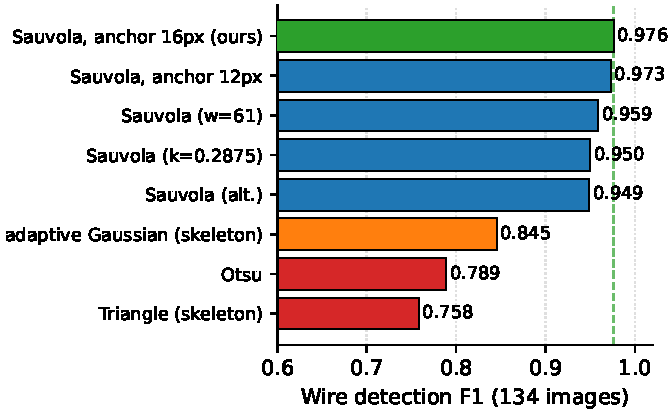
\includegraphics[width=\columnwidth]{figures/wire_benchmark.pdf}
\caption{Wire detection F1 across thresholding methods and pipeline variants (134 images). Our configuration, Sauvola binarization with a 16\,px anchor filter, achieves F1~=~0.976; Otsu and triangle thresholding both degrade sharply.}
\label{fig:wire_benchmark}
\end{figure}

\begin{table}[htbp]
\caption{Wire Detection Performance (134 images)}
\label{tab:wire_benchmark}
\begin{center}
\begin{tabular}{lccc}
\toprule
\textbf{Configuration} & \textbf{F1} & \textbf{Prec} & \textbf{Rec} \\
\midrule
Sauvola + anchor 16\,px (ours) & \textbf{0.976} & 0.973 & 0.978 \\
Sauvola + anchor 12\,px & 0.973 & 0.974 & 0.972 \\
Sauvola ($w{=}61$) + anchor 12\,px & 0.959 & 0.944 & 0.974 \\
Sauvola ($k{=}0.2875$) + anchor 14\,px & 0.950 & 0.921 & 0.980 \\
Otsu threshold + CCL & 0.789 & 0.796 & 0.783 \\
\bottomrule
\end{tabular}
\end{center}
\end{table}

Median F1 across the benchmark set is 1.000, and 87\% of images score F1~$\geq$~0.90. Sauvola adaptive binarization beats every alternative we tried: Otsu gives F1~=~0.789, adaptive Gaussian F1~=~0.845. Component occlusion also matters: skip it, and component internals (text, symbols, internal wiring) generate hundreds of false wire detections.

\subsection{Join Strategy Comparison}

Table~\ref{tab:join_leaderboard} and Figure~\ref{fig:join_comparison} compare joining strategies on the synthetic framework (15 circuits $\times$ 8 seeds, mean F1 over error levels L1--L4).

\begin{table}[htbp]
\caption{Join Strategy Leaderboard (Synthetic Eval)}
\label{tab:join_leaderboard}
\begin{center}
\footnotesize
\setlength{\tabcolsep}{4pt}
\begin{tabular}{lccccc}
\toprule
\textbf{Strategy} & \textbf{L0} & \textbf{L1} & \textbf{L2} & \textbf{L3} & \textbf{L4} \\
\midrule
Scale-rel.\ graph + completion (ours) & 1.00 & 1.00 & 1.00 & \textbf{0.96} & \textbf{0.95} \\
Rescue graph + completion & 1.00 & 1.00 & 1.00 & 0.95 & 0.94 \\
Rescue graph (base) & 1.00 & 1.00 & 1.00 & 0.94 & 0.90 \\
Scale-rel.\ graph (base) & 1.00 & 1.00 & 1.00 & 0.94 & 0.85 \\
Radius union-find (legacy) & 1.00 & 0.97 & 0.90 & 0.56 & 0.36 \\
Nearest-pin + bbox anchor & 1.00 & 0.97 & 0.89 & 0.38 & 0.32 \\
\bottomrule
\end{tabular}
\end{center}
\end{table}

The completion-based strategies are the most robust of the lot, holding F1~$\geq$~0.94 at the highest error severity (L4) against F1~=~0.36 for the legacy radius union-find baseline, a 2.6$\times$ improvement. The radius join's transitive grabbing over-merges catastrophically under noise: at L4 it shorts multiple components onto the same net. But the endpoint-graph base joins are already far more robust than the radius join on their own, reaching F1~=~0.90 at L4 (Table~\ref{tab:join_leaderboard}). Degree-budget completion adds a further $+0.05$ on top of the strongest of these by recovering dropped connections that the base graph join leaves floating, and its per-pin edge budget keeps precision from slipping. Pairing that completion with the high-precision scale-relative base, the scale-relative completion join used throughout, gives the best synthetic robustness (0.95 at L4) and, more to the point, the best \emph{real-image} connectivity (Section~\ref{sec:real_eval}). The large gap shown is against the legacy radius join; against the strongest prior graph join the improvement is smaller but holds at every severity level. We leave out two intermediate variants for readability, since their synthetic scores fall within rounding of rows already shown: nearest-pin without anchoring, and the scale-relative base with end-extension but no dead-end rescue.

\begin{figure*}[t]
\centering
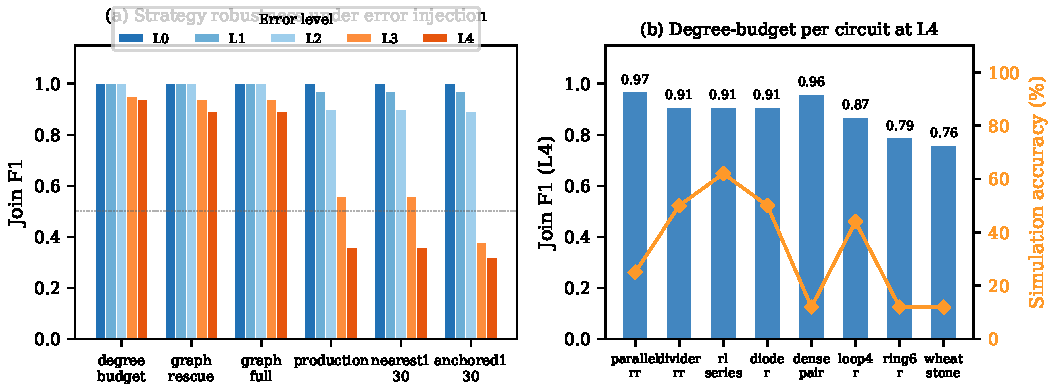
\includegraphics[width=\textwidth]{figures/join_comparison.pdf}
\caption{(a)~Join strategy robustness under error injection (15 circuits $\times$ 8 seeds): bars give mean connectivity F1 at each severity level (L0--L4, dark to light to red). The completion-based strategies (left) stay near 1.0, while the radius union-find and nearest-pin baselines (right) collapse at L3--L4. (b)~The scale-relative completion join per circuit at L4 (16 seeds): bars are connectivity F1, and the orange line is simulation accuracy. Errors cause fragmentation rather than shorts, so precision stays high (Table~\ref{tab:per_circuit}); the balanced Wheatstone bridge is the hardest case.}
\label{fig:join_comparison}
\end{figure*}

\subsection{Real-Image Net-Level Evaluation}
\label{sec:real_eval}

The synthetic results measure robustness under a parametric error model, but they say nothing about real detector output. To close that gap we built, to our knowledge, the first \emph{human-verified net-level} ground truth for hand-drawn circuits: 31 CGHD-1152 images in which every electrical net was traced and confirmed by a human annotator using a purpose-built verification tool. One of our comparison points is a vision-language model (Section~\ref{sec:vlm_results}), so it matters that the human, not any model, is the verifier of record; the answer key is independent of every method under test. Net-level proposals were bootstrapped with a conservative endpoint-graph join over the dataset's perfect wire labels and then hand-corrected. During verification the human repeatedly caught cases where the bootstrap join had wrongly split a single rail into two, and we further re-validate every conclusion against the independently authored synthetic ground truth to rule out residual bootstrap bias. Connectivity is scored as component-pair F1 restricted to SPICE-active components, the same metric used in the synthetic evaluation.

Table~\ref{tab:real_join} reports every registered join strategy on the verified set, all run on the pipeline's own detected wires. Our primary metric is micro-averaged (pair-pooled) component-pair F1, so a dense 14-component board contributes in proportion to its connections rather than counting the same as a 3-component one; macro (mean per-image) F1 is listed alongside for reference. The best configuration, the scale-relative completion join (degree-budget completion on top of a high-precision scale-relative endpoint-graph base), reaches micro-F1~=~0.890 (P~=~0.92, R~=~0.86; 95\% bootstrap CI [0.855, 0.924]), ahead of the prior default that pairs the same completion with the rescue base (0.829) and the radius union-find join (0.667) (Figure~\ref{fig:real_join_fig}). The gain over rescue-based completion traces back to a cleaner base: the rescue base's 12\,px end-extension and dead-end rescue over-reach on noisy detected wires and cost precision, while the scale-relative base keeps precision high and lets the bounded completion recover recall on its own. A reach sweep shows the F1 plateau is broad across reach $3$--$5\times s$ (macro-F1 0.898--0.903 over that range), so this setting is robust rather than tuned to a spike. Confidence intervals are wide at $N=31$ and the per-strategy intervals overlap, but the ranking is stable and is corroborated on the independently authored synthetic suite (Table~\ref{tab:join_leaderboard}).

\begin{table}[htbp]
\caption{Join Strategy and Baseline Comparison on Human-Verified Net-Level Ground Truth (31 real images, detected wires). Primary metric is micro-averaged (pair-pooled) component-pair F1; macro (mean per-image) F1 is shown for reference.}
\label{tab:real_join}
\begin{center}
\footnotesize
\setlength{\tabcolsep}{4pt}
\begin{tabular}{lcccc}
\toprule
\textbf{Method} & \textbf{F1} & \textbf{Prec} & \textbf{Rec} & \textbf{F1$_{\text{macro}}$} \\
\midrule
\multicolumn{5}{l}{\emph{Deterministic joins (ours and ablations)}} \\
Scale-rel.\ graph + completion (ours) & \textbf{0.890} & 0.919 & 0.864 & \textbf{0.901} \\
Rescue graph + completion (prior) & 0.829 & 0.789 & 0.874 & 0.853 \\
Scale-rel.\ graph (base) & 0.816 & 0.929 & 0.727 & 0.838 \\
Rescue graph (base) & 0.787 & 0.811 & 0.764 & 0.813 \\
Radius union-find (legacy) & 0.667 & 0.698 & 0.638 & 0.674 \\
\midrule
\multicolumn{5}{l}{\emph{Classical deterministic baselines (identical detected wires)}} \\
Hough + proximity (best) & 0.805 & 0.750 & 0.868 & 0.847 \\
Connected-components (best) & 0.624 & 0.965 & 0.461 & 0.611 \\
\midrule
\multicolumn{5}{l}{\emph{Reference (non-deterministic / oracle wires)}} \\
VLM (Claude Opus~4.8) & 0.923 & 0.970 & 0.880 & 0.949 \\
Scale-rel.\ + completion, perfect wires & 0.890 & 0.913 & 0.868 & 0.916 \\
\bottomrule
\end{tabular}
\end{center}
\end{table}

\begin{figure}[t]
\centering
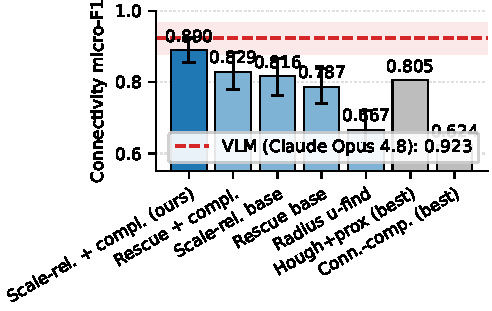
\includegraphics[width=\columnwidth]{figures/real_join_comparison.pdf}
\caption{Micro-averaged connectivity F1 on the 31-image human-verified net-level benchmark (component-pair metric). Our scale-relative completion join leads every deterministic strategy and the classical Hough and connected-component baselines, all run on identical detected wires. The dashed line marks a strong VLM (Claude Opus 4.8) evaluated on the same 31 images, from which our join is statistically indistinguishable (paired micro-F1 difference $+0.033$, 95\% bootstrap CI $[-0.009, +0.078]$) while being deterministic, structurally valid, and orders of magnitude cheaper. Error bars are 95\% bootstrap CIs.}
\label{fig:real_join_fig}
\end{figure}

This settles a question left open by earlier work on the pipeline: against bootstrapped pilot labels, degree-budget completion had \emph{not} consistently beaten its base join, but against human-verified ground truth it clearly does (micro-F1 0.829 vs 0.787 for the rescue base alone), and the scale-relative variant does better still. The same ordering shows up on the authored synthetic suite (Table~\ref{tab:join_leaderboard}), where the scale-relative completion join also ranks first, so this is not an artifact of how the net-level labels were bootstrapped.

The connectivity recipe used by most prior image-to-netlist systems erases the component boxes and reads nets off the connected components, or contours, of the residual wire pixels. SINA~\cite{sina2026}, the concurrent contour-based node detector of Peker et al.~\cite{peker2026}, AMSnet~\cite{amsnet2025}, and the Bayer instance-segmentation pipeline~\cite{instanceseg2023} all use it, and it was designed for clean printed schematics. On hand-drawn photographs it has no good operating point: pencil-stroke fragmentation splits each net into many components (F1~$<$~0.25 at any sensible morphological gap-bridging setting), and only pathological closing, which effectively merges by proximity, lifts recall, at a steep cost to precision. To isolate the join algorithm from binarization quality we ran connected-component labeling on our \emph{own} detected wire segments, the same input our join receives, and its best configuration reaches only micro-F1~=~0.624 (recall collapses to 0.46, since the blobs short or drop most nets), against 0.890 for the endpoint-graph join (Table~\ref{tab:real_join}). A stronger classical alternative, Hough-transform line detection~\cite{duda1972hough} followed by proximity linking, does better because line fitting denoises the fragmented strokes; it reaches micro-F1~=~0.805 at its best-tuned linking tolerance, but still trails our join by 0.085 and at markedly lower precision. Every baseline is reported at its best configuration over a tolerance sweep, so these numbers are upper bounds on what the classical recipes can do. Explicit typed-endpoint reasoning with bounded completion beats both blob/contour connectivity and line-primitive proximity tracing.

We also tried running five public image-to-netlist systems end-to-end on our hand-drawn benchmark, and none could be fairly applied. The classical printed-schematic interpreter of Kelly and Cole~\cite{kelly2024digitizing} installs and runs, but on hand-drawn scans it over-segments wires into spurious components and recovers almost no connectivity: a domain-transfer failure. Netlistify~\cite{netlistify2025} reproduces on its own printed AMS test data, which we ran end-to-end with the released model, but its active model lacks the diode, inductor, and IC classes our circuits contain, and its connectivity model is trained on printed thin-line appearance, so it has no way to represent hand-drawn discrete circuits. Masala-CHAI~\cite{masalachai2024} hands connectivity off to a proprietary LLM behind a paid API, which is close in spirit to our own VLM experiment (Section~\ref{sec:vlm_results}) rather than a deterministic algorithm. SINA's~\cite{sina2026} anonymized code archive would not extract, and CircuitNet~\cite{circuitnet} ships only Colab notebooks with no released weights. The survey itself is informative: no prior system offers a deterministic, hand-drawn-ready connectivity module, which leaves the controlled CCL and Hough baselines above, both run on our identical detected wires, as the fair points of comparison, and our join beats both.

Swapping the dataset's perfect wire labels in for detected wires leaves micro-F1 unchanged at 0.890, and raises macro-F1 only from 0.901 to 0.916 (Table~\ref{tab:real_join}); the wire detector is responsible for essentially none of the pair-weighted F1 gap. What error remains is intrinsic join ambiguity on hand-drawn geometry, not wire detection, which fits with the 0.976 wire-detection F1 reported earlier (Table~\ref{tab:wire_benchmark}). The join degrades only gently with circuit size: per-image F1 falls from 0.94 on circuits with $\leq$6 components to 0.86 above that, a weak correlation ($r=-0.19$), and precision stays high throughout. That is a different failure mode from the VLM, whose recall drops on the largest boards while its precision holds (Section~\ref{sec:vlm_results}).

\begin{figure}[t]
\centering
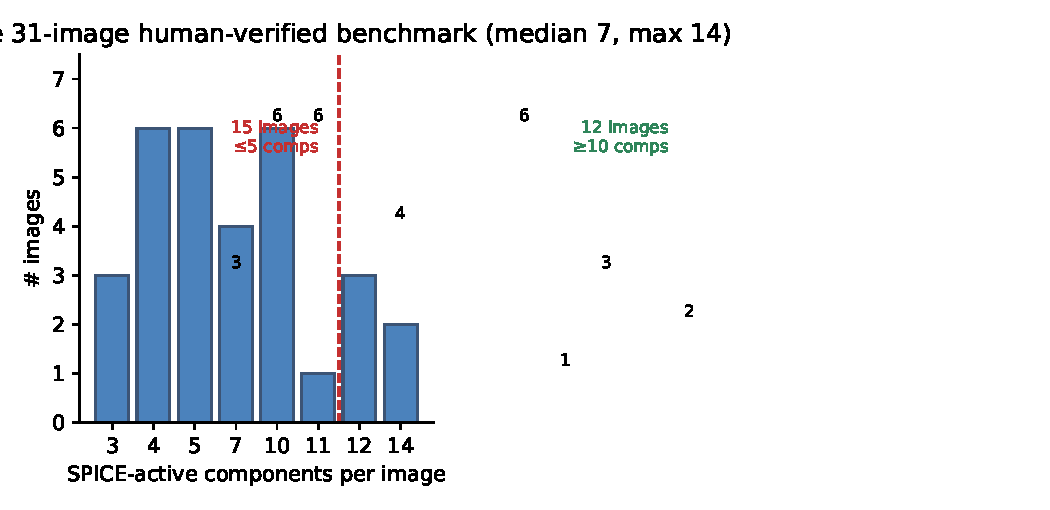
\includegraphics[width=0.82\textwidth]{figures/complexity_histogram.pdf}
\caption{Complexity of the 31-image human-verified benchmark, in SPICE-active components per image. The distribution is bimodal, not ``dominated by 3--6 component topologies'': 15 images have $\leq$5 components and 12 have $\geq$10 (median 7, max 14), so the benchmark includes a real share of larger boards, and the per-image size--F1 analysis below reports how performance holds up on them.}
\label{fig:complexity_hist}
\end{figure}

\subsection{Per-Drafter Consistency}
To check generalization across drawing styles within the corpus, Table~\ref{tab:per_drafter} breaks down the headline join (scale-relative completion) by the CGHD drafter who drew each schematic. We recovered drafter identity from the CGHD-1152 source tree: 16 of 31 images by direct filename match, and the rest inferred from the dataset's documented 12-circuits-per-drafter block structure, which fits every directly verified drafter with zero exceptions. Four drafters contribute at least four benchmark images each; micro-F1 across them ranges 0.854--0.987, with no drafter showing catastrophic failure. That supports generalization across drafters within this corpus, though the cell sizes are too small to draw strong statistical conclusions.

\begin{table}[htbp]
\caption{Join micro-F1 (scale-relative completion) by CGHD drafter on the 31-image human-verified benchmark.}
\label{tab:per_drafter}
\centering
\begin{tabular}{lcccc}
\hline
Drafter & $n$ images & micro-F1 & macro-F1 & TP/FP/FN \\
\hline
drafter\_1  & 7 & 0.933 & 0.907 & 56/6/2 \\
drafter\_2  & 5 & 0.854 & 0.874 & 85/14/15 \\
drafter\_10 & 5 & 0.987 & 0.995 & 37/1/0 \\
drafter\_12 & 4 & 0.913 & 0.938 & 21/0/4 \\
\hline
Overall    & 31 & 0.890 & 0.901 & 418/37/66 \\
\hline
\end{tabular}
\end{table}

\subsection{Per-Circuit Analysis}

Table~\ref{tab:per_circuit} breaks down the scale-relative completion join's performance across eight representative circuits from the 15-circuit synthetic corpus at L4 (extreme error injection, 16 seeds).

\begin{table}[htbp]
\caption{Scale-Relative Completion Join Performance per Circuit at L4 (16 seeds)}
\label{tab:per_circuit}
\begin{center}
\begin{tabular}{lrrrr}
\toprule
\textbf{Circuit} & \textbf{Comps} & \textbf{F1} & \textbf{Prec} & \textbf{Sim.\ acc.} \\
\midrule
Parallel R--R & 3 & 1.00 & 1.00 & 25\% \\
R--R divider & 3 & 0.99 & 1.00 & 69\% \\
RL series & 3 & 0.99 & 1.00 & 81\% \\
Diode--R loop & 3 & 0.99 & 1.00 & 69\% \\
Dual R loops & 4 & 0.93 & 0.90 & 12\% \\
4-component loop & 4 & 0.94 & 0.91 & 56\% \\
Wheatstone bridge & 6 & 0.82 & 0.85 & 6\% \\
6-component ring & 6 & 0.95 & 0.92 & 50\% \\
\bottomrule
\end{tabular}
\end{center}
\end{table}

Precision stays high ($\geq$~0.85) across every circuit even at L4: errors cause \emph{fragmentation}, dropped connections, rather than \emph{shorts}, false merges. The Wheatstone bridge is the hardest topology (F1~=~0.82): its balanced arms make the inferred node structure sensitive to a single misplaced connection, and simulation accuracy falls to 6\%.

\subsection{VLM Connectivity Experiment}
\label{sec:vlm_results}

Section~\ref{sec:vlm_connectivity} argues that an explicit geometric model solves connectivity better than a VLM left to its own devices; to put a number on that claim, we ran a first-party experiment with a strong general VLM (Claude Opus~4.8). We match component priors by giving the VLM exactly what the join receives, the scanned image plus the same ground-truth component boxes labelled by index, and ask it to return, as JSON, the sets of component terminals that share an electrical node; we score the resulting component-pairs with the same metric used elsewhere. Each image goes through an independent, context-free model call, one per image, so no answer leaks between circuits, and the human stays the verifier of record, not the model. On a clean synthetic control (15 authored circuits) the VLM scores F1~=~0.99, so it clearly understands the task and the symbol set. Across all 31 real scans, scored against the human-verified net-level ground truth, it reaches micro-F1~=~0.923 (P~=~0.97, R~=~0.88; macro-F1~=~0.949).

So the VLM edges out our deterministic join on aggregate, 0.923 versus 0.890 micro-F1, but the gap is not statistically significant: a paired bootstrap over the 31 images puts the difference at $+0.033$ with a 95\% CI of $[-0.009, +0.078]$, which includes zero. Two further findings qualify the comparison. First, the VLM's accuracy falls off with circuit complexity. It is exact (F1~=~1.00) on 21 of the 31 circuits, including 14 of the 15 small 3--5-component cases (the exception is C138\_D1\_P3), but on the largest boards it systematically \emph{omits} connections, with recall falling to 0.63--0.68 on three of the four largest boards (C77, C84, C66), which is exactly where a netlist error costs the most. Its recall degrades, not its precision, which stays high at 0.97 micro, so the failure mode is dropped nets rather than shorts. The macro-F1 (0.949) is inflated by the many easy small circuits, which is why we treat the pair-weighted micro-F1 as primary. Second, the cost and the shape of the output differ from the geometric pipeline: each image burns on the order of $10^5$ tokens, the result is free-form text rather than a structured netlist, and nothing in the model guarantees electrical validity, for instance that a two-terminal component is not shorted. Our geometric join is statistically indistinguishable from the VLM on these circuits while being deterministic, two to three orders of magnitude cheaper, guaranteed against shorts by the self-loop guard, and simulatable as SPICE syntax by construction. We treat the VLM here as an upper reference for what a frontier model can do, not as a connectivity module to ship: an explicit model matches its accuracy and also gives a deployed digitizer the determinism, low cost, and structural validity it needs.

\section{Discussion}

The endpoint-graph model resolves an ambiguity that radius-based methods cannot even see: by representing both wire endpoints and component pins as nodes with typed edges, it tells apart a wire that merely \emph{passes near} a component (endpoint--wire-body edge) from one that actually \emph{connects to} it (endpoint--pin edge with directional preference). Component-first assignment adds a further constraint: a wire has to reach a component's pin, not just its bounding box.

Degree-budget completion exists because detector noise is unavoidable: even a wire detector that is 97.6\% accurate drops about 2\% of wire endpoints, and those are exactly the connections that matter most for getting the simulation right. The $b$-matching formulation caps the damage a mis-detection can do, since each floating pin gets at most one recovery edge, and the self-loop guard rules out the catastrophic short-circuit failures that plague unconstrained approaches.

The human-verified net-level evaluation is novel for hand-drawn circuits, but it still covers only 31 images, so the 95\% bootstrap confidence intervals on per-strategy F1 are wide ($\pm$0.03--0.05) and overlap between adjacent strategies. The top ranking is consistent and corroborated by the independently authored synthetic suite, but separating the closely ranked configurations will need broader annotation. The net-level labels themselves were bootstrapped by a conservative endpoint-graph join over perfect wires and then corrected by hand; to address the concern that this favors graph-based methods, we validate on synthetic ground truth authored entirely from scratch, and the same ranking holds there too. The evaluation draws on a single hand-drawn corpus (CGHD-1152), so generalization to other drawing styles, capture conditions, and printed schematics is still an open question. The pipeline only emits SPICE-active netlist pins for device classes with connectivity-verified pin templates (resistor, capacitor, inductor, diode, transistor, voltage source, and IC-as-black-box); more complex devices such as transformers, thyristors, optocouplers, triacs, relays, and switches are detected and located but their pin relationships are not extracted, so they sit outside both the net-level benchmark and netlist emission. The VLM connectivity comparison relies on a single frontier model (Claude Opus~4.8) on the same 31 images; testing more models and prompting strategies is future work. Component detection itself has room to improve, at 88.5\% mean average precision (mAP@0.5), particularly on crossovers, where recall is 70.7\%. The component-detection model was trained on CGHD-1152 after excluding drafter\_0, whose drawing style diverged markedly from the rest; that shrinks the training set but avoids domain-shift artifacts from an outlier style. Finally, the synthetic error model is a first-pass approximation of detector noise rather than a calibrated fit; now that the real-image net-level metric exists, calibrating it against the measured detector failure distribution is a natural next step.

\section{Conclusion}

We built a complete deterministic pipeline for hand-drawn circuit digitization: an occlusion-first wire extractor that produces an endpoint representation, a two-stage endpoint-graph join, and, to our knowledge, the first human-verified net-level connectivity benchmark for hand-drawn circuits. The endpoint-graph join with degree-budget completion is the most robust strategy under synthetic error injection (F1~=~0.95 at the highest severity against 0.36 for the radius baseline). Paired with a high-precision scale-relative base, it reaches connectivity micro-F1~=~0.890 on our 31-image, CGHD-1152-sourced benchmark against human-verified ground truth, ahead of the prior completion default (0.83) and every deterministic baseline we tested, including the connected-component net-tracing recipe used by recent systems (0.62) and a Hough-plus-proximity line tracer (0.81), all on identical detected wires. Running the join on perfect wires does not move micro-F1 at all, which places the bottleneck squarely in the join rather than in wire detection. A first-party experiment with a frontier VLM reaches 0.923 on the same images, a gap from our join that is not statistically significant (paired 95\% CI $[-0.009, +0.078]$), but at two to three orders of magnitude higher cost and without structurally valid, machine-checkable output. That comparison is the case for the explicit geometric design. What is left: scaling the human-verified benchmark, calibrating the synthetic error model against the measured detector distribution, and extending coverage to devices outside the simulatable set.

% Funding moved to \tfootnote in the front matter (IEEE Access convention).

\section*{Acknowledgment}
The authors used Claude Opus 4.8 (Anthropic) to assist with grammar and language editing of the manuscript and as a programming assistant during development of the pipeline and evaluation code. This assistance is distinct from the VLM connectivity experiment in Section~\ref{sec:vlm_results}, where the same model is an evaluation subject. All methods, experiments, and conclusions are the authors' own, and the authors reviewed and take full responsibility for the entire content of this article.

\section*{Data and Code Availability}
The pipeline, evaluation scripts, synthetic-circuit generator, the 31-image
human-verified net-level ground truth (\texttt{ground\_truth/real\_nets\_verified.json}),
the net-level verification tool used to produce it, the join-strategy and
connected-component baseline benchmarks, and the Claude-VLM connectivity harness are
available at
\url{https://github.com/boscochanam/circuit-digitization}. The component-detection model
is available at \url{https://huggingface.co/boscochanam/circuit-component-detector}, trained
on the CGHD-1152 dataset~\cite{bayer2021cghd}.

\begin{thebibliography}{00}
\bibitem{bayer2021cghd} F.~Thoma, J.~Bayer, Y.~Li, and A.~Dengel, ``A public ground-truth dataset for handwritten circuit diagram images,'' in \textit{Proc. Int. Conf. Document Analysis and Recognition (ICDAR)}, 2021, pp.~20--27. [Online]. Available: \url{https://doi.org/10.1007/978-3-030-86198-8_2}
\bibitem{kelly2024digitizing} C.~R.~Kelly and J.~M.~Cole, ``Digitizing images of electrical-circuit schematics,'' \textit{APL Mach. Learn.}, vol.~2, no.~1, p.~016109, 2024.
\bibitem{sina2026} S.~Aldowaish, Y.~Karumanchi, K.-C.~Chiang, S.~Noorzad, and M.~Fayazi, ``SINA: A circuit schematic image-to-netlist generator using artificial intelligence,'' in \textit{Proc. Design, Automation \& Test in Europe Conf. (DATE)}, 2026. [Online]. Available: \url{https://doi.org/10.23919/DATE69613.2026.11539285}
\bibitem{masalachai2024} J.~Bhandari, V.~Bhat, Y.~He, H.~Rahmani, S.~Garg, and R.~Karri, ``Masala-CHAI: A large-scale SPICE netlist dataset for analog circuits by harnessing AI,'' arXiv:2411.14299, 2024.
\bibitem{peker2026} \"{O}.~B.~Peker, E.~Toker, D.~\"{O}cal, T.~Dalyan, E.~Afacan, and Y.~D.~G\"{o}kdel, ``A fully automated SPICE-compatible netlist extraction from image using deep learning and image preprocessing techniques,'' \textit{IEEE Access}, vol.~14, pp.~19750--19765, 2026, doi: 10.1109/ACCESS.2026.3656316.
\bibitem{instanceseg2023} J.~Bayer, A.~Roy, and A.~Dengel, ``Instance segmentation based graph extraction for handwritten circuit diagram images,'' in \textit{Proc. 12th Int. Conf. Pattern Recognition Applications and Methods (ICPRAM)}, 2023. [Online]. Available: \url{https://doi.org/10.5220/0011752600003411}
\bibitem{handdrawn2021} R.~R.~Reddy and M.~R.~Panicker, ``Hand-drawn electrical circuit recognition using object detection and node recognition,'' \textit{SN Comput. Sci.}, vol.~3, no.~3, p.~244, 2022. arXiv:2106.11559.
\bibitem{juhccr2025} A.~Roy, S.~Pani, S.~Malakar, and R.~Sarkar, ``JUHCCR-v1: A database for hand-drawn electrical and electronics circuit component recognition,'' \textit{Sci. Rep.}, vol.~15, art.~no.~22404, 2025, doi: 10.1038/s41598-025-22404-5.
\bibitem{redmon2016yolo} J.~Redmon, S.~Divvala, R.~Girshick, and A.~Farhadi, ``You only look once: Unified, real-time object detection,'' in \textit{Proc. IEEE Conf. Computer Vision and Pattern Recognition (CVPR)}, 2016, pp.~779--788.
\bibitem{jocher2023yolo} G.~Jocher, A.~Chaurasia, and J.~Qiu, ``Ultralytics YOLO,'' 2023. [Online]. Available: \url{https://github.com/ultralytics/ultralytics}
\bibitem{smith2007tesseract} R.~Smith, ``An overview of the Tesseract OCR engine,'' in \textit{Proc. 9th Int. Conf. Document Analysis and Recognition (ICDAR)}, 2007, pp.~629--633.
\bibitem{nagel1973spice} L.~W.~Nagel and D.~O.~Pederson, ``SPICE: Simulation program with integrated circuit emphasis,'' Electron. Res. Lab., Univ. California, Berkeley, Memo. ERL-M382, 1973.
\bibitem{amsnet2025} Y.~Shi, Z.~Tao, Y.~Gao, L.~Huang, H.~Wang, Z.~Yu, T.-J.~Lin, and L.~He, ``AMSnet 2.0: A large AMS database with AI segmentation for net detection,'' arXiv:2505.09155, 2025.
\bibitem{amsbench2025} Y.~Shi, Z.~Zhang, H.~Wang, Z.~Tao, Z.~Li, B.~Chen, Y.~Wang, Z.~Huang, X.~Liu, Q.~Chen, Z.~Yu, T.-J.~Lin, and L.~He, ``AMSbench: A comprehensive benchmark for evaluating MLLM capabilities in AMS circuits,'' arXiv:2505.24138, 2025.
\bibitem{diagramnet2026} J.~Lou, R.~Xu, J.~Li, J.~Pi, R.~Tao, W.~Fan, X.~Tan, G.~Luo, and Y.~Lin, ``DiagramNet: An end-to-end recognition framework and dataset for non-standard system-level diagrams,'' arXiv:2605.01338, 2026.
\bibitem{llm4eda2024} R.~Zhong, X.~Du, S.~Kai, Z.~Tang, S.~Xu, H.-L.~Zhen, J.~Hao, Q.~Xu, M.~Yuan, and J.~Yan, ``LLM4EDA: Emerging progress in large language models for electronic design automation,'' arXiv:2401.12224, 2024.
\bibitem{kulkarni2025enhancing} S.~Kulkarni \textit{et~al.}, ``Enhancing circuit diagram understanding via near sight correction using VLMs,'' in \textit{Proc. ICCV Workshops}, 2025.
\bibitem{duda1972hough} R.~O.~Duda and P.~E.~Hart, ``Use of the Hough transformation to detect lines and curves in pictures,'' \textit{Commun. ACM}, vol.~15, no.~1, pp.~11--15, 1972.
\bibitem{sauvola2000} J.~Sauvola and M.~Pietik\"{a}inen, ``Adaptive document image binarization,'' \textit{Pattern Recognit.}, vol.~33, no.~2, pp.~225--236, 2000.
\bibitem{he2017ccl} L.~He, X.~Ren, Q.~Gao, X.~Zhao, B.~Yao, and Y.~Chao, ``The connected-component labeling problem: A review of state-of-the-art algorithms,'' \textit{Pattern Recognit.}, vol.~70, pp.~25--43, 2017.
\bibitem{tarjan1975union} R.~E.~Tarjan, ``Efficiency of a good but not linear set union algorithm,'' \textit{J. ACM}, vol.~22, no.~2, pp.~215--225, 1975.
\bibitem{kuhn1955} H.~W.~Kuhn, ``The Hungarian method for the assignment problem,'' \textit{Naval Res. Logist. Quart.}, vol.~2, no.~1--2, pp.~83--97, 1955.
\bibitem{schrijver2003combinatorial} A.~Schrijver, \textit{Combinatorial Optimization: Polyhedra and Efficiency}. Berlin, Germany: Springer, 2003.
\bibitem{alrahis2021gnn} L.~Alrahis, A.~Sengupta, J.~Knechtel, S.~S.~Gharibeh, O.~S.~Unsal, M.~E.~Acar, and H.~Najjar, ``GNN-RE: Graph neural networks for reverse engineering of gate-level netlists,'' in \textit{Proc. IEEE/ACM Int. Conf. Computer-Aided Design (ICCAD)}, 2021, pp.~1--9.
\bibitem{netlistify2025} C.-Y.~Huang, H.-I.~Chen, H.-W.~Ho, P.-H.~Kang, M.~P.-H.~Lin, W.-H.~Liu, and H.~Ren, ``Netlistify: Transforming circuit schematics into netlists with deep learning,'' in \textit{Proc. ACM/IEEE Symp. Machine Learning for CAD (MLCAD)}, 2025.
\bibitem{circuitnet} ``CircuitNet: A hand-drawn schematic sketch recognizer and converter,'' GitHub repository (user aaanthonyyy), 2024. [Online]. Available: \url{https://github.com/aaanthonyyy/CircuitNet}
\end{thebibliography}

% ---- Author biographies (IEEE Access requires one for EVERY author) ----
% The class opens each bio with "\vskip \@IEEEBIOskipN plus 1fil", so leftover
% column space stretches into large gaps between bios. Cap that stretch and
% let spare space fall to the column bottom instead.
\makeatletter
% The env takes an optional arg, so its body lives in the internal
% macro \csname\string\IEEEbiography\endcsname, not \IEEEbiography.
\expandafter\patchcmd\csname\string\IEEEbiography\endcsname%
  {\vskip \@IEEEBIOskipN plus 1fil minus 0\baselineskip}%
  {\vskip \@IEEEBIOskipN plus 0.5\baselineskip minus 0\baselineskip}%
  {}{\typeout{WARNING: IEEEbiography spacing patch did not apply}}
\makeatother
\raggedbottom
\begin{IEEEbiography}[{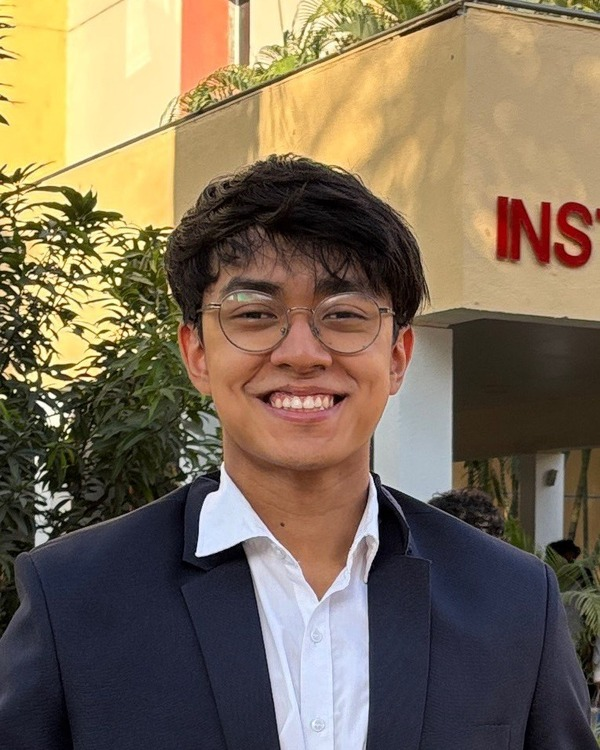
\includegraphics[width=1in,height=1.25in,clip,keepaspectratio]{figures/authors/chanam.jpg}}]{Bosco Chanam}
received the B.Tech.\ degree in Computer Science and Engineering from the Symbiosis Institute of Technology (SIT), Pune, India. He is currently an AI/ML Engineer at the AI Incubation Centre at Bharat Forge (Kalyani Group), Pune, India. His professional and research interests include computer vision, edge AI optimization, and robotics. Mr.~Chanam has co-authored research in natural language processing benchmarking, published in the \textit{International Journal of Fuzzy Logic and Intelligent Systems}.
\end{IEEEbiography}

\begin{IEEEbiography}[{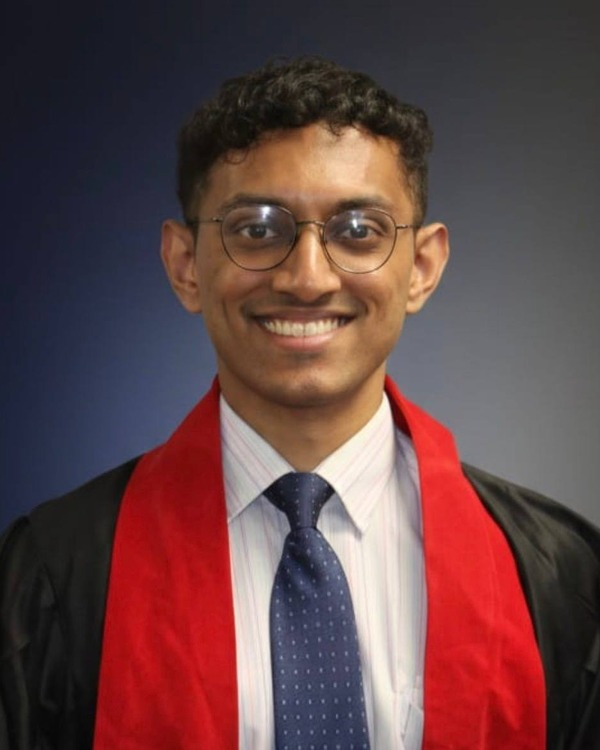
\includegraphics[width=1in,height=1.25in,clip,keepaspectratio]{figures/authors/dcosta.jpg}}]{Chris Dcosta}
received the B.Tech.\ degree in Computer Science and Engineering with Honors in Artificial Intelligence and Machine Learning from the Symbiosis Institute of Technology (SIT), Pune, India. His research interests include computer vision, machine learning, natural language processing, and deep learning.
\end{IEEEbiography}

\begin{IEEEbiography}[{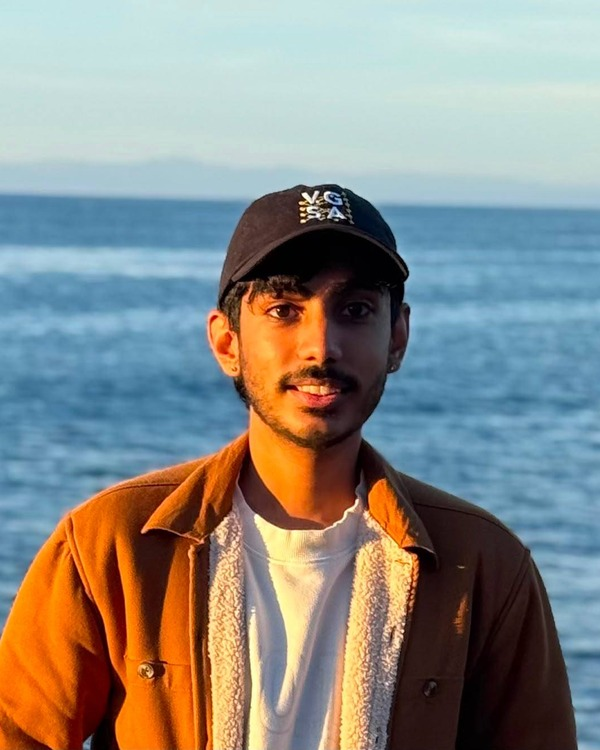
\includegraphics[width=1in,height=1.25in,clip,keepaspectratio]{figures/authors/talupuri.jpg}}]{Pranavesh Kumar Talupuri}
is with the Department of Computer Science, University of Southern California, Los Angeles, CA, USA. His research interests include machine learning, deep learning, and computer vision.
\end{IEEEbiography}

\begin{IEEEbiography}[{
\includegraphics[width=1in,height=1.25in,clip,keepaspectratio]{figures/authors/chiwhane.jpg}}]{Shwetambari Chiwhane}
holds a B.E. in Computer Science and Engineering from Sant Gadge
Baba Amravati University, Amravati, India, and an M.Tech. in Computer Science and Engineering
from Dr. Babasaheb Technological University, Lonere, India. She earned her PhD in Computer
Engineering specializing from Bharath Institute of Higher Education and Research, Chennai,
India. Presently, she serves as an Assistant Professor in the Department of Computer Science and
Engineering at Symbiosis Institute of Technology, Symbiosis International (Deemed University),
Pune, India, gathering over two decades of teaching and research expertise. She is life member of
ISTE.

Her contributions extend beyond academia; she has contributed as a reviewer for various
international conferences. Dr. Shwetambari's research expertise is evident with her receiving many
publications. She has authored over 35 research articles in various international and national
conferences and journals. Her professional engagements include roles such as NAAC, NBA,
among others.

Recognized as a PhD guide in Symbiosis International (Deemed University), Presently she is
guiding 4 research scholar and she has guided more than 100 undergraduate students for their
research endeavors. Her current research interests revolve around Image Processing, Computer
Vision, Artificial Intelligence and Machine Learning.
\end{IEEEbiography}

\begin{IEEEbiography}[{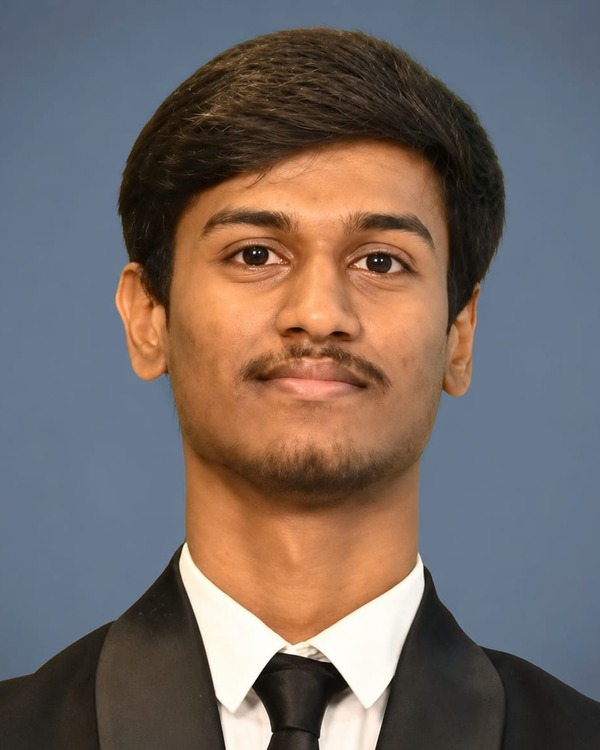
\includegraphics[width=1in,height=1.25in,clip,keepaspectratio]{figures/authors/singh.jpg}}]{Ashay Kumar Singh}
received the B.Tech.\ degree in Computer Science and Engineering from the Symbiosis Institute of Technology (SIT), Pune, India. His research interests lie in machine learning, computer vision, Retrieval-Augmented Generation (RAG), optical character recognition (OCR), and multimodal AI.
\end{IEEEbiography}

\begin{IEEEbiography}[{
\includegraphics[width=1in,height=1.25in,clip,keepaspectratio]{figures/authors/das.jpg}}]{Arghadeep Das}
received the B.Tech.\ degree in Computer Science and Engineering from the Symbiosis Institute of Technology (SIT), Pune, India. His research interests include reinforcement learning, world models, computer vision, 3D rendering, agentic AI, embodied AI, robotics, and machine learning.
\end{IEEEbiography}

\EOD

\end{document}
